% ======================================================================
%  CHƯƠNG 4 — THỰC NGHIỆM VÀ PHÂN TÍCH KẾT QUẢ
%  Yêu cầu (mục 2.5): >= 2 bộ dữ liệu chuẩn; độ đo phù hợp; so sánh >= 2 baseline;
%  bảng + biểu đồ; phân tích; ablation study.
%  Lưu ý trung thực: các số liệu dưới đây là KẾT QUẢ SƠ BỘ (ngân sách 30s trên
%  máy cục bộ). Lần chạy đầy đủ trên 20 bộ dữ liệu (môi trường Docker/Linux) đang
%  được hoàn tất; các ô [ ] là chỗ điền số liệu cuối cùng.
%  Độ dài tham khảo: >= 10 trang.
% ======================================================================
\chapter{Thực nghiệm và phân tích kết quả}
\label{ch:thucnghiem}

\section{Bộ dữ liệu}
\label{sec:dulieu}
Đồ án sử dụng hai nhóm dữ liệu. \emph{Nhóm thứ nhất} là bộ sưu tập gồm 20 bộ dữ
liệu công khai thu thập từ Kaggle (mỗi thành viên chuẩn bị 5 bộ), cân bằng giữa
bài toán phân lớp và hồi quy, dùng cho lần chạy so sánh đầy đủ. \emph{Nhóm thứ
hai} là các bộ dữ liệu chuẩn nhỏ, dùng cho lần chạy sơ bộ nhằm kiểm chứng quy
trình end-to-end. Bảng~\ref{tab:dulieu} thống kê ba bộ dữ liệu của lần chạy sơ bộ.
Việc nạp và quản lý dữ liệu được thực hiện qua giao diện của hệ thống
(Hình~\ref{fig:console-datasets}).

\begin{figure}[H]
    \centering
    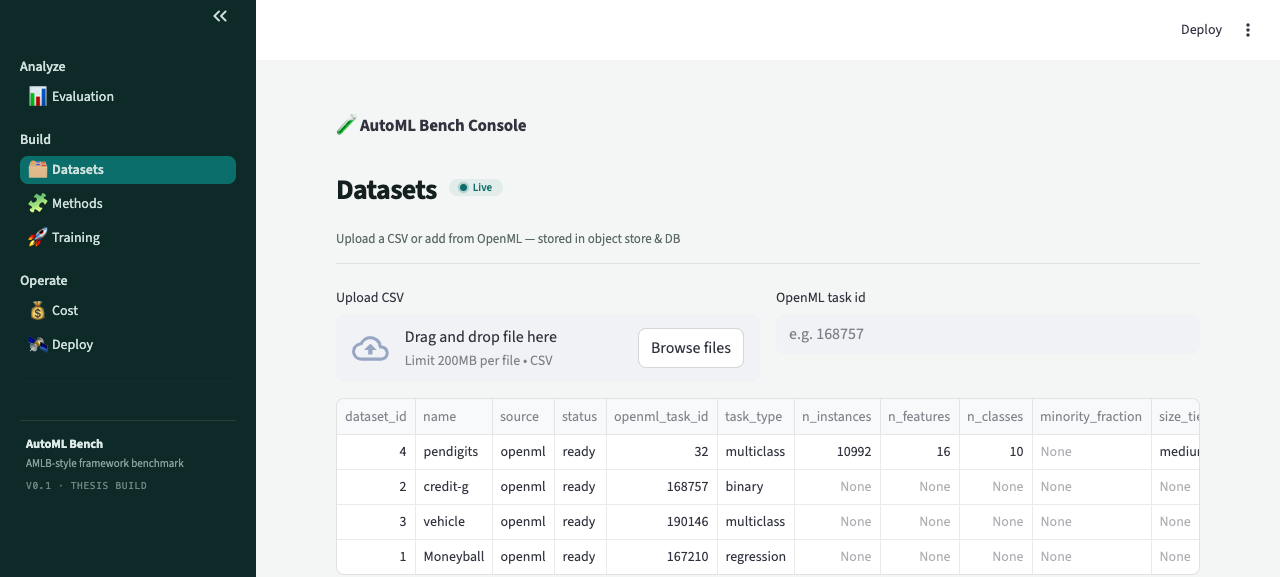
\includegraphics[width=0.9\linewidth]{image/console-datasets.png}
    \caption{Trang Datasets: nạp dữ liệu từ tệp CSV, tác vụ OpenML hoặc liên kết
    Kaggle công khai; mỗi bộ được ghi nhận kèm loại, nguồn và trạng thái.}
    \label{fig:console-datasets}
\end{figure}

\begin{table}[H]
  \centering
  \small
  \caption{Ba bộ dữ liệu dùng trong lần chạy sơ bộ.}
  \label{tab:dulieu}
  \renewcommand{\arraystretch}{1.2}
  \begin{tabularx}{\linewidth}{@{}l l l X@{}}
    \toprule
    \textbf{Bộ dữ liệu} & \textbf{Loại tác vụ} & \textbf{Độ đo} & \textbf{Ghi chú} \\
    \midrule
    breast\_cancer       & Phân lớp nhị phân & AUC       & Chẩn đoán u lành/ác. \\
    wine                 & Phân lớp đa lớp   & log-loss  & Phân loại ba giống rượu vang. \\
    california\_housing  & Hồi quy           & RMSE      & Dự đoán giá nhà. \\
    \bottomrule
  \end{tabularx}
\end{table}

\noindent Bảng~\ref{tab:dulieu-full} là khung thống kê cho bộ 20 bộ dữ liệu Kaggle
(điền khi hoàn tất thu thập).

\begin{table}[H]
  \centering
  \small
  \caption{Thống kê bộ 20 bộ dữ liệu Kaggle (khung điền).}
  \label{tab:dulieu-full}
  \renewcommand{\arraystretch}{1.15}
  \begin{tabularx}{\linewidth}{@{}l c c c X@{}}
    \toprule
    \textbf{Bộ dữ liệu} & \textbf{Tác vụ} & \textbf{Số mẫu} & \textbf{Số đặc trưng} & \textbf{Nguồn} \\
    \midrule
    {[}\ldots{]} & {[}\ldots{]} & {[}\ldots{]} & {[}\ldots{]} & Kaggle: {[}liên kết{]} \\
    \multicolumn{5}{c}{\textit{\ldots\ (tổng cộng 20 bộ: 10 phân lớp, 10 hồi quy)}} \\
    \bottomrule
  \end{tabularx}
\end{table}

\section{Thiết lập thực nghiệm}
\label{sec:thietlap}
\textbf{Thư viện so sánh:} FLAML, H2O~AutoML và AutoGluon. \\
\textbf{Baseline:} rừng ngẫu nhiên (\textit{RandomForest}) và bộ dự đoán hằng
(\textit{constantpredictor}) --- hai baseline được AMLB cung cấp sẵn, dùng làm mốc
dưới để kiểm tra xem một thư viện có thực sự ``học'' được gì hay không. \\
\textbf{Ràng buộc tài nguyên:} theo ba mức của AMLB --- \texttt{smoke} (1 fold,
60 giây, 4 nhân), \texttt{1h} (10 fold, 3600 giây, 8 nhân) và \texttt{4h} (10
fold, 14400 giây, 8 nhân). Lần chạy sơ bộ dùng ngân sách 30 giây/fold. \\
\textbf{Môi trường:} mỗi thư viện chạy trong ảnh Docker \texttt{automlbenchmark/*}
riêng để bảo đảm môi trường đồng nhất; siêu dữ liệu và kết quả lưu trên
PostgreSQL, tệp dữ liệu và dự đoán lưu trên MinIO. Người dùng chọn thư viện, bộ
dữ liệu và ngân sách rồi khởi chạy trực tiếp từ trang Training
(Hình~\ref{fig:console-training}).

\begin{figure}[H]
    \centering
    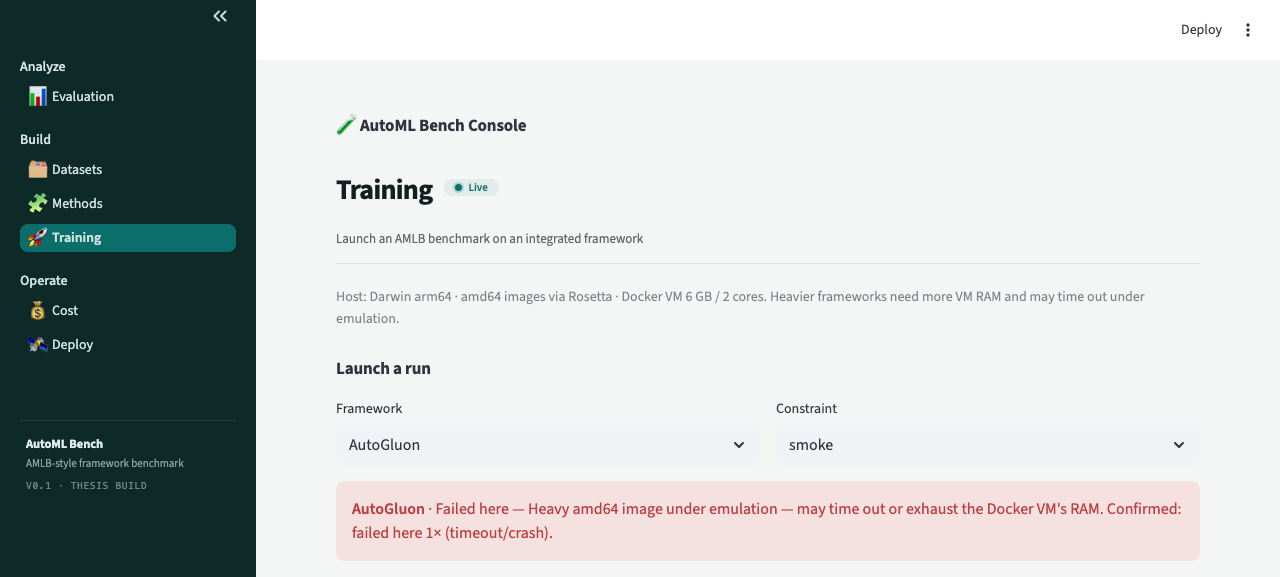
\includegraphics[width=0.9\linewidth]{image/console-training.png}
    \caption{Trang Training: chọn thư viện, bộ dữ liệu và ngân sách để khởi chạy
    một lần đánh giá trong Docker; các tác vụ tự động cập nhật trạng thái.}
    \label{fig:console-training}
\end{figure}

\section{Độ đo đánh giá}
\label{sec:dodo}
Nhóm dùng AUC cho phân lớp nhị phân, log-loss cho phân lớp đa lớp và RMSE cho hồi
quy (định nghĩa và ví dụ tính đã trình bày ở Mục~\ref{sec:dodo-lythuyet}, Ví
dụ~\ref{vd:rmse}). Kết quả tổng hợp được quy về \emph{thứ hạng trung bình} theo
công thức ở Mục~\ref{sec:giaothuc} để so sánh xuyên suốt các loại độ đo.

\section{Kết quả sơ bộ và xếp hạng}
\label{sec:ketqua}
Bảng~\ref{tab:ketqua} trình bày điểm số và chi phí thời gian của ba thư viện trên
ba bộ dữ liệu ở ngân sách 30 giây/fold. Đây là kết quả \emph{sơ bộ} nhằm kiểm
chứng quy trình; lần chạy đầy đủ trên 20 bộ dữ liệu đang được hoàn tất.

\begin{table}[H]
  \centering
  \small
  \caption{Kết quả sơ bộ: điểm số (và thời gian chạy, giây) ở ngân sách 30s/fold.
  Giá trị tốt nhất mỗi hàng được in đậm.}
  \label{tab:ketqua}
  \renewcommand{\arraystretch}{1.25}
  \begin{tabularx}{\linewidth}{@{}>{\raggedright\arraybackslash}X c c c@{}}
    \toprule
    \textbf{Bộ dữ liệu (độ đo)} & \textbf{FLAML} & \textbf{AutoGluon} & \textbf{H2O} \\
    \midrule
    breast\_cancer (AUC $\uparrow$)
        & \makecell{0.9957\\(68.2s)} & \makecell{0.9961\\(37.4s)} & \makecell{\textbf{0.9974}\\(57.4s)} \\
    california\_housing (RMSE $\downarrow$)
        & \makecell{0.4693\\(33.8s)} & \makecell{\textbf{0.4320}\\(31.5s)} & \makecell{0.4389\\(125.9s)} \\
    wine (log-loss $\downarrow$)
        & \makecell{0.0487\\(161.4s)} & \makecell{0.0099\\(31.5s)} & \makecell{\textbf{0.0038}\\(130.7s)} \\
    \midrule
    \textbf{Thứ hạng trung bình} & 3.00 & 1.67 & \textbf{1.33} \\
    \bottomrule
  \end{tabularx}
\end{table}

Cách tính thứ hạng trung bình đã được minh hoạ ở Ví dụ~\ref{vd:rank}. Hình
\ref{fig:rank} trực quan hoá thứ hạng này (thấp hơn là tốt hơn).

\begin{figure}[H]
    \centering
    \begin{tikzpicture}
    \begin{axis}[
        width=0.72\linewidth, height=5.2cm,
        ybar, bar width=20pt,
        symbolic x coords={H2O, AutoGluon, FLAML},
        xtick=data, ymin=0, ymax=3.4,
        ylabel={Thứ hạng TB ($\downarrow$)},
        nodes near coords, enlarge x limits=0.35]
      \addplot coordinates {(H2O, 1.33) (AutoGluon, 1.67) (FLAML, 3.00)};
    \end{axis}
    \end{tikzpicture}
    \caption{Thứ hạng trung bình của ba thư viện trên lần chạy sơ bộ (càng thấp
    càng tốt).}
    \label{fig:rank}
\end{figure}

Ở ngân sách nhỏ này, H2O và AutoGluon nhỉnh hơn FLAML về chất lượng, nhưng FLAML
và AutoGluon thường hoàn tất nhanh hơn --- cho thấy sự \emph{đánh đổi giữa chất
lượng và thời gian}. Bảng~\ref{tab:full} là khung tổng hợp cho lần chạy đầy đủ.

\begin{table}[H]
  \centering
  \small
  \caption{Kết quả tổng hợp trên 20 bộ dữ liệu (khung điền cho lần chạy đầy đủ).}
  \label{tab:full}
  \renewcommand{\arraystretch}{1.2}
  \begin{tabularx}{\linewidth}{@{}X c c c c@{}}
    \toprule
    \textbf{Thư viện} & \textbf{Thắng phân lớp} & \textbf{Thắng hồi quy} & \textbf{Thứ hạng TB} & \textbf{Thời gian TB} \\
    \midrule
    FLAML      & [\,] & [\,] & [\,] & [\,] \\
    H2O AutoML & [\,] & [\,] & [\,] & [\,] \\
    AutoGluon  & [\,] & [\,] & [\,] & [\,] \\
    RandomForest (baseline)     & [\,] & [\,] & [\,] & [\,] \\
    constantpredictor (baseline)& [\,] & [\,] & [\,] & [\,] \\
    \bottomrule
  \end{tabularx}
\end{table}

\section{So sánh với baseline}
\label{sec:baseline}
Theo giao thức AMLB, mọi thư viện được đối chiếu với hai baseline. Một thư viện
AutoML chỉ thực sự có giá trị nếu vượt rõ rệt bộ dự đoán hằng và ít nhất không
thua rừng ngẫu nhiên. [Điền phân tích sau lần chạy đầy đủ: thư viện nào vượt
baseline trên loại tác vụ nào, mức vượt bao nhiêu.]

\section{Nghiên cứu loại bỏ thành phần (ablation)}
\label{sec:ablation}
Nhóm khảo sát ảnh hưởng của \emph{ngân sách thời gian} --- yếu tố tác động mạnh
tới AutoML --- bằng cách chạy cùng cấu hình ở các mức ngân sách khác nhau và quan
sát biến thiên của chất lượng và thứ hạng (Bảng~\ref{tab:ablation}).

\begin{table}[H]
  \centering
  \small
  \caption{Ablation theo ngân sách thời gian (thứ hạng trung bình).}
  \label{tab:ablation}
  \renewcommand{\arraystretch}{1.2}
  \begin{tabular}{@{}lccc@{}}
    \toprule
    \textbf{Ngân sách} & \textbf{FLAML} & \textbf{AutoGluon} & \textbf{H2O} \\
    \midrule
    30 giây/fold (sơ bộ) & 3.00 & 1.67 & 1.33 \\
    smoke (60s, 1 fold)  & [\,] & [\,] & [\,] \\
    1h (3600s, 10 fold)  & [\,] & [\,] & [\,] \\
    \bottomrule
  \end{tabular}
\end{table}

[Phân tích: khi tăng ngân sách, thứ hạng giữa các thư viện thay đổi ra sao; thư
viện nào tận dụng ngân sách lớn tốt hơn.]

\section{Phân tích lỗi và thảo luận}
\label{sec:phantichloi}
Việc ghi nhận thất bại (thay vì bỏ qua) giúp phân tích các nguyên nhân thực tế
cản trở một so sánh công bằng. Trên máy cục bộ macOS (arm64, Python~3.9), nhóm
quan sát các lỗi sau khi cố gắng chạy trực tiếp không dùng Docker:
\begin{itemize}
    \item \textbf{Lệch phiên bản thư viện phụ thuộc:} \texttt{TunedRandomForest}
    lỗi do \texttt{scikit-learn 1.6.1} đã loại bỏ hàm \texttt{\_check\_fit\_params}
    mà AMLB còn gọi --- một minh hoạ điển hình cho việc môi trường không đồng nhất
    phá vỡ tính tái lập.
    \item \textbf{Thiếu thư viện hệ thống:} FLAML cần \texttt{libomp} cho XGBoost
    (khắc phục bằng cách cài đặt bổ sung).
    \item \textbf{Kịch bản cài đặt hướng Linux:} H2O và AutoGluon dùng script cài
    đặt cho Linux, thất bại trên macOS (\texttt{AutoGluon setup.sh} thoát mã 127).
\end{itemize}
Bốn trong sáu bộ chạy thất bại khi chạy cục bộ. Quan sát này chính là lý do đồ án
chọn chạy lần đánh giá đầy đủ trong \emph{môi trường Docker/Linux đồng nhất}: chỉ
khi cô lập môi trường thì so sánh giữa H2O, FLAML và AutoGluon mới thực sự công
bằng. Hình~\ref{fig:console-methods} minh hoạ trang quản lý và tích hợp thư viện
của hệ thống, nơi trạng thái tích hợp và mức tương thích theo máy được hiển thị
trung thực.

\begin{figure}[H]
    \centering
    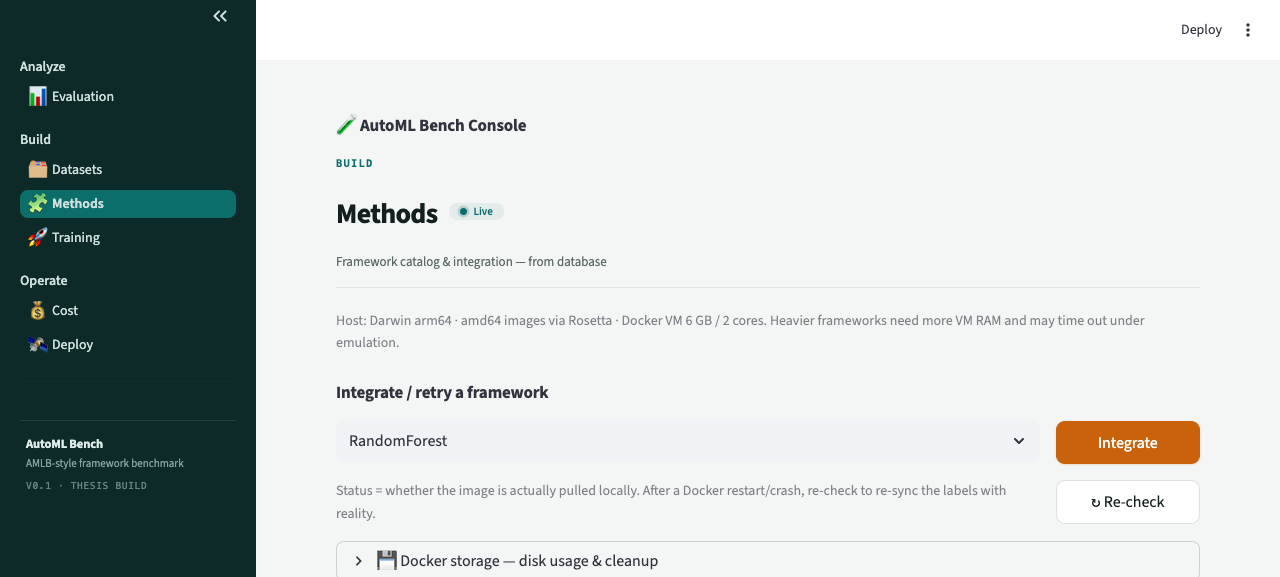
\includegraphics[width=0.9\linewidth]{image/console-methods.png}
    \caption{Trang Methods: danh mục thư viện AutoML với trạng thái tích hợp, phù
    hiệu tương thích theo máy và dung lượng Docker.}
    \label{fig:console-methods}
\end{figure}

Tổng hợp lại, kết quả sơ bộ đã kiểm chứng quy trình end-to-end (chạy $\to$ chấm
điểm $\to$ xếp hạng) dưới một giao thức thống nhất; phần phân tích lỗi cho thấy
giá trị của việc ghi nhận thất bại và cô lập môi trường. Kết quả đầy đủ trên 20
bộ dữ liệu sẽ củng cố các nhận định về sự đánh đổi chất lượng -- chi phí giữa các
thư viện.
